 % Use only LaTeX2e, calling the article.cls class and 12-point type.

\documentclass[12pt]{article}

\usepackage{amsmath,amssymb}
\usepackage{hyperref}
\usepackage[normalem]{ulem}
\usepackage{graphicx}
\usepackage{lscape}

% The following parameters seem to provide a reasonable page setup.
\topmargin 0.0cm
\oddsidemargin 0.2cm
\textwidth 16cm 
\textheight 21cm
\footskip 1.0cm

% Include your paper's title here

\title{Lagrange Geometry Class} 
\author{Aleksejs Fomins}
\date{}

%%%%%%%%%%%%%%%%% END OF PREAMBLE %%%%%%%%%%%%%%%%

\begin{document} 

% Double-space the manuscript.
% \baselineskip24pt

% Make the title.
\maketitle 

\section{Preliminaries}

\subsection{Initialization}

LagrangeGeometry class is initialized with a geometry type/reference element, set of interpolatory vertices of the element, and the interpolation order. These are used to initialize a CurvilinearElementInterpolator class, which interpolates over vertices and provides an analytical map from global to local coordinates $\vec{p}(\vec{u})$. This map can either be provided analytically as a vector of polynomials, or immediately evaluated within the Interpolator class which is a little faster, as lagrange polynomials are also given explicitly.

\section{Point Location}

\subsection{Point location with respect to a plane}

Assume that a plane is given by 3 coordinates $\vec{a}, \vec{b}, \vec{c}$, and we would like to check on which side of this plane the point $\vec{p}$ is. This is uniquely given by a function
\begin{equation}
\label{equation-point-plane-test}
	ptest(\vec{a}, \vec{b}, \vec{c}, \vec{p}) = \mathrm{sgn} \{ \det (\vec{a} - \vec{p}, \vec{b} - \vec{p}, \vec{c} - \vec{p}) \}
\end{equation}
\noindent
This function takes values $1,-1$ for corresponding sides of the plane, and $0$ if the point is on the plane.

\subsection{Locating the element the given global coordinate belongs to}
\label{subsection-locating-element}

\noindent
Current convention: loop over all elements in the mesh, check if the point is inside the element using the method below. \\


\noindent
This method has $O(1)$ initialization cost, but $O(N) * ins$ query cost, which becomes wastefully slow as the number of points to locate grows. Here $ins$ is the cost of $is\_inside$ method, which has constant complexity if the query point is far away from the triangle, but requires an iterative method for nearby methods.

\noindent
There are two ways one can implement the above idea: \\
\textbf{First method:}
\begin{enumerate}
	\item Iterate over all elements, use linear $check\_inside()$
	\item For the element for which linear $check\_inside() = true$ run the nonlinear $check\_inside()$
	\item If the nonlinear $check\_inside() = false$, recursively do nonlinear $check\_inside()$ on the neighbors of the element.
\end{enumerate}
\textbf{Second method:}
\begin{enumerate}
	\item Iterate over all elements, use nonlinear $check\_inside()$
\end{enumerate}
\noindent
The first method is better, because it will on average have less runs of the iterative method, as if the point is located in a linear element, it has high probability of being located inside the nonlinear element with the same corners. \\

\noindent
An improvement would be to implement an OCTree, which will have a recursively-refined cubic mesh over the tetrahedral one, and upon initialization would place each of the tetrahedrons recursively within one or more leafs of the tree. Thus the initialization cost would be $O(N \log(N))$, and the cost of a single query $O(\log(N)) + M * inc$, where $M$ is the number of neighbors an element has. This is a considerable improvement for large number of queries. \\

\noindent
\textbf{OCTree method}:
\begin{enumerate}
	\item Construct the OCTree - grid the domain, build the hierarchical tree, place the correct element labels into each leaf
	\item For each query, locate the leaf the query point corresponds to
	\item Proceed by using one of the above methods on the element set of the leaf
\end{enumerate}

\begin{figure}[hp]
    \centering
    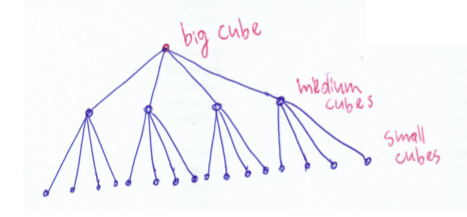
\includegraphics[scale=0.7]{doc-pics/pic-octree-3.png}
	\caption{OcTree internal structure}    
    
    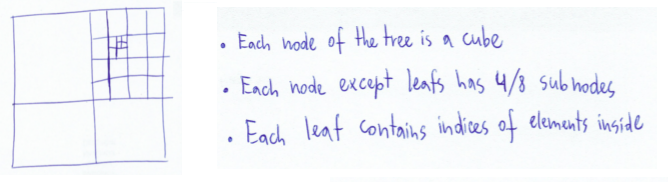
\includegraphics[scale=0.7]{doc-pics/pic-octree-1.png}
	\caption{OcTree grid}    
	
    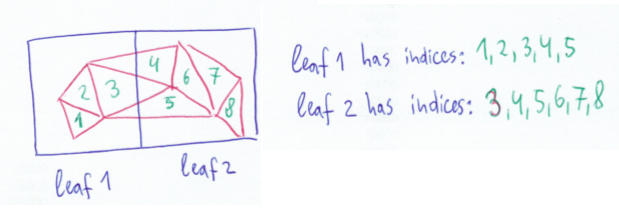
\includegraphics[scale=0.7]{doc-pics/pic-octree-2.png}
	\caption{OcTree partition of elements}    
    %\caption{Awesome Image}
    %\label{fig:awesome_image}
\end{figure}


\noindent
How does this work with parallel processing?

\subsection{Checking if a global coordinate is inside a given element (straight sided)}
\label{subsection-isinside-linear}

\noindent
For straight-sided elements the conversion between global and local coordinates is 1-to-1 in the whole space.
Therefore, it is sufficient to find the corresponding local coordinate and use the $referenceelement$ method $checkInside$. \\

\noindent
For example, for a simplex the $is\_inside(u,v,w)$ for local coordinates $(u,v,w)$ looks like 
\[u \geq 0\ \&\ v \geq 0\ \&\ w \geq 0,\ \&\ u+v+w \leq 0. \]

\noindent
Naturally, the global-local map has a finite precision, therefore the $checkInside$ method corrects for that by having a small tolerance for above inequalities, thus avoiding the case where a boundary point would be considered outside both neighboring elements because of numerical errors.


\subsection{Checking if a global coordinate is inside a given element (curvilinear elements)}
\label{subsection-isinside-nonlinear}

\noindent
This method is only defined if ($(dim_{elem} = dim_{world})$). For discussion see the $local()$ method discussion.

\noindent
In principle, this method requires an iterative solver, but first we run two simpler tests which immediately identify some of the points inside or outside of the element. \\

\noindent
\textbf{Far-point test}:
\begin{enumerate}
	\item Define linear center $\vec{p}_{CoM}$ of an element as the center of mass of its corners.
	\item Define the radius of an element $R$ as the largest distance between $\vec{p}_{CoM}$ and a point $\vec{p}_b$ on its boundary
	\item Define linear radius $R_{lin}$ to be the largest distance between $\vec{p}_{CoM}$ and one of the corners of the element. It can be shown that $R_{lin} = \frac{\sqrt{dim^2 + dim - 1}}{dim + 1} $, which is $\{ \frac{1}{2}, \frac{\sqrt{5}}{3}, \frac{\sqrt{11}}{4} \}$ for dimensions $\{1,2,3\}$.
	\item Demand that for all sensible curvilinear elements, $R$ should be bounded by some scaling of $R_{lin}$. For example, we can require that $R \leq 2 R_{lin}$, which would mean that all poins of every element should be entirely contained within $2 R_{lin}$ of its center. A more precise prefactor could be calculated from curvature constants of the bounaries of the element (max over the boundary of some expr. involving derivatives of interpolatory polynomials).
	\item Thus, if $|\vec{p}_{CoM} - \vec{p}|_2 > 2 R_{lin}$, we can immediately report that $\vec{p}$ is outside the element.
\end{enumerate}

\noindent
\textbf{Global Barycentric Coordinate test}:
\begin{enumerate}
	\item Define a global barycentric coordinate as the area enclosed by one curved boundary of the element, the point of interest, and the straight-sided boundaries that connect the point of interest and the corners of the curved boundary.
		\subitem - for 2D triangle, a barycentric coordinate is given by
		\[B = \frac{1}{2}\int_0^1 (\vec{p}(u) - \vec{p}_0) \times \partial_u \vec{p}(u) du\]
		as derived from triangle area $S = \frac{1}{2} \vec{a} \times \vec{b}$. Here $\vec{p}_0$ is the coordinate of interest.
		\subitem - for 3D tetrahedron, a barycentric coordinate is given by
		\[B = \frac{1}{3}\int_0^1 \int_0^{1-u} (\vec{p}(u,v) - \vec{p}_0) \cdot (\partial_u \vec{p}(u,v) \times \partial_v \vec{p}(u,v)) du\]
		as derived from tetrahedron volume area $V = \frac{1}{6} \vec{a} \cdot (\vec{b} \times \vec{c})$.
		Note that there is an additional factor of 2 in the barycentric equation, because triangular grid only covers half of the triangle, whereas
		parallelogram grid covers the whole (check figure \ref{fig:barycentric_coordinate_calculation})

\begin{figure}[!htb]
    \centering	
    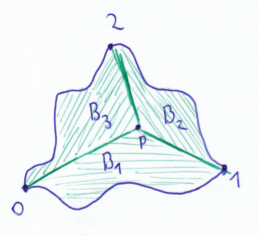
\includegraphics[scale=0.7]{doc-pics/pic-barycentric-curvilinear-definition.png}
    \caption{Definition of Barycentric Curvilinear Coordinates}
    %\label{fig:awesome_image}
\end{figure}

	\item For linear elements, the sum of barycentric coordinates always equals the total volume of the element for internal points, and is larger than that for external points. This is not true for non-convex elements, as the sum may be larger than the volume even for internal points. The method can not be improved by considering the sign of the barycentric coordinate based on the orientation of the boundary, as it is the same for internal and external points of the concave surface.
	\item Thus, if the sum of global barycentric coordinates is equal to the volume of the element, the point is automatically inside the element, otherwise we remain uncertain.
			
\end{enumerate}

\begin{figure}[!htb]
    \centering	
    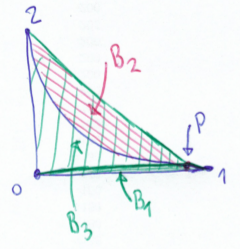
\includegraphics[scale=0.7]{doc-pics/pic-barycentric-problem-1.png}
    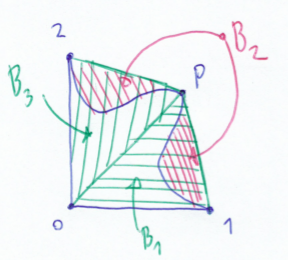
\includegraphics[scale=0.7]{doc-pics/pic-barycentric-problem-2.png}
    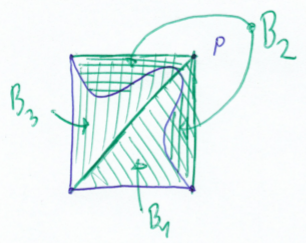
\includegraphics[scale=0.7]{doc-pics/pic-barycentric-problem-3.png}
    \caption{Problem cases with Barycentric Curvilinear coordinates}
    %\label{fig:awesome_image}
\end{figure}

\noindent
If both the above tests do not give a conclusive result, we need to use Global-To-Local mapping, and then $checkInside$ for the local coordinate. The challenges of this approach are described in the corresponding section. \\

\noindent
\textbf{Current Implementation: } There is no $is\_inside()$ method, only $local()$ method. Local method returns false if the point is not inside the element, and returns true and the correct local coordinate if it is. If the answer is true, we have to calculate the local coordinate anyway to make sure, makes sense to return it not to calculate it twice.

\begin{figure}[p]
    \centering
    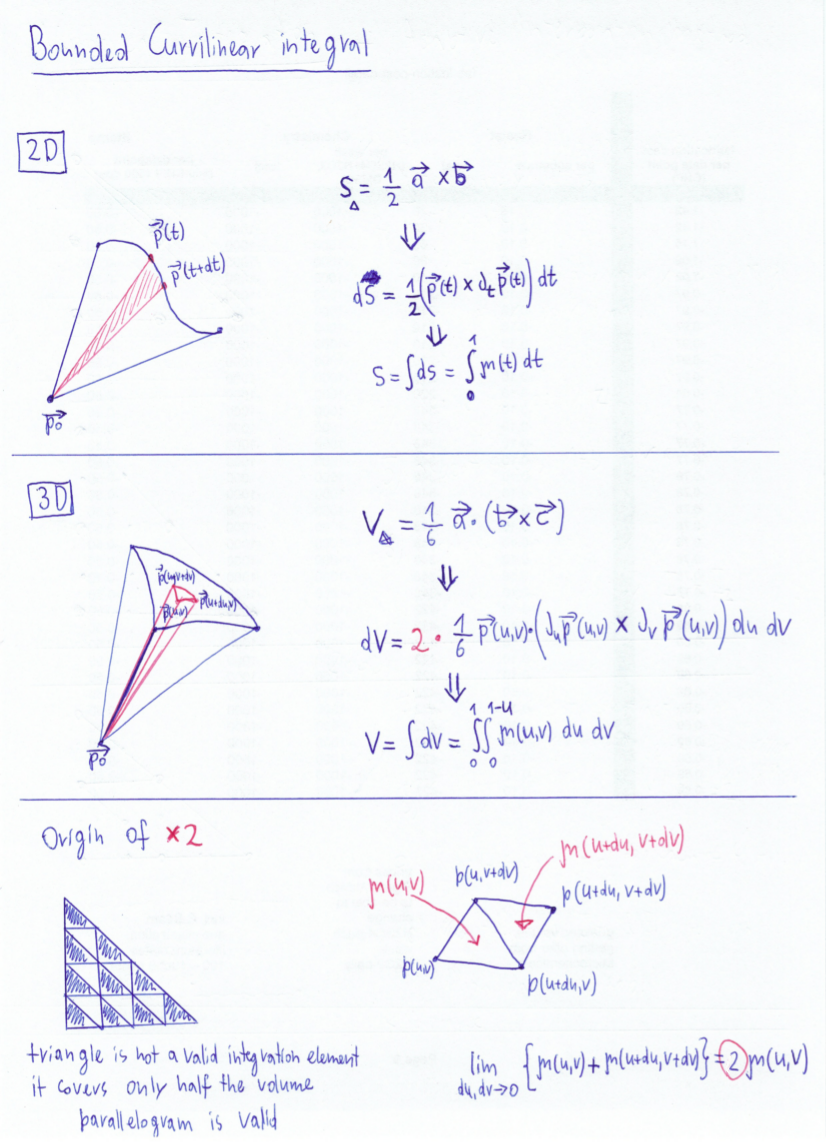
\includegraphics[scale=0.7]{doc-pics/pic-bounded-curvilinear-integral.png}
    \caption{Barycentric Coordinate Calculation}
    \label{fig:barycentric_coordinate_calculation}
\end{figure}


\section{Coordinate transformation}

\subsection{Jacobian and JacobianInverse}

From the ElementInterpolation class one can request a complete analytical interpolatory polynomial for each of the coordinates $x,y,z$. Then one uses the polynomial methods differentiate and evaluate to calculate $J_{ij} = \partial_i p_j (u,v,w) |_{u_0, v_0, w_0}$. The inverse and determinant are obtained using JacobianInverse class, which uses MatrixHelper to invert matrix and calculate the pseudodeterminant $\sqrt{\det(JJ^T)}$. \\

\subsection{Local-to-Global mapping}

The global coordinate is obtained by calling the corresponding method $realCoordinate()$ of the Interpolator class. It evaluates a linear combination of lagrange polynomials for each coordinate.

\subsection{Global-to-Local mapping}

This method finds local coordinate within this element from a given global coordinate. The $is\_inside()$ method is part of this method, as it returns false if the point is not within the element, and true + the local coordinate, if the point is. \\

\noindent
After a discussion the following was agreed on:
\begin{itemize}
	\item $local()$ method is not defined outside the element. Even for most simple polynomial maps, there exist global coordinates which do not correspond to any local coordinate at all. For example, $x^2$ is a perfectly valid local-to-global map for an edge defined on $[0,1]$, however, no local coordinate at all corresponds to the global coordinate $-1$. Therefore, if we have high evidence that a point is located outside the element, we only report that it is outside and do not report any local coordinate. As the local coordinate is found using an iterative process, it needs to have a termination condition, because, given that a local coordinate of interest does not exist, the method will not converge.
	\item $local()$ method is only defined when $(dim_{elem} = dim_{world})$. For inequal dimensions, disregarding the question being a challenging computational task, it is also meaningless. The probability that a randomly selected point would belong to a manifold of dimension lower than the world dimension is negligibly small. If the point is non-random, it must have been generated using a local-to-global map of one of the elements, in which case there are much more cost-efficient ways of tracing it back, for example, by storing the local coordinate mapped.
\end{itemize}

\noindent
Even considering the two above simplifications, this is still a very tricky problem. Since the map from local to global is polynomial, it is in principle non-invertible, at least not in terms of standard functions \\

\noindent
It can be guaranteed that the map is one-to-one within the element, otherwise the the real element geometry would be self-intersecting, which should be ensured by GMSH when selecting interpolation points. However, there are no obvious reasons why the geometry should not be self-intersecting outside the element, which means that the map need not be one-to-one outside the element. \\

\noindent
For obvious reasons we will not solve the problem directly, as searching for roots of a system of polynomial equations with several parameters is a very challenging task. Instead we minimize the two-norm \[\vec{r} = \mathrm{argmin} \{ |\vec{p}(\vec{r}) - \vec{p}_0 |^2 \}. \] We think that the problem should not have local extrema inside the element, because that is equivalent to having $\det J = 0$. However, it will most likely have local extrema outside the element (especially for higher orders). The solutions proposed:
\begin{itemize}
	\item Currently Dune uses Newton's method \[\vec{r}_{n+1} = \vec{r}_n + \mathrm{LinSolve}(J(\vec{r}_n), \vec{p}(\vec{r}_n) ). \] Since the mapping is 1-to-1 inside the element, it should definitely not have minima and maxima, not sure about extrema. Therefore Newton's method should converge to the right solution if the starting point is selected inside the element, for example its center.
	
	\item Termination condition:
		- The iterative solution should not be strongly outside the element for some iteration, if the true solution is inside. Therefore, we terminate if at any point $|\vec{p}_{CoM} - \vec{p}|_2 > 4 R_{lin}$, using the notation from $is\_inside()$ descriotion.
	
	\item This method may fail if there indeed is an extrema inside the element, and after an unlucky step it is thrown out of the element even though the correct solution is inside. Thus, if the method fails to find the point within the element and its neighbors this way, it may make sense to try several starting locations within each tetrahedron hoping to avoid the extrema.
\end{itemize}

\section{Integration}

It is necessary to integrate scalar and vector functions over an element. \\

\noindent
In original strategy (Multilinear Geometry using Gaussian quadrature), the geometry only needed to provide an integration element, the integration itself was performed in dervied classes outside DUNE. However, for the special case of integrating a polynomial function over the element, the resulting integral is frequently possible to calculate analytically. Such integration requires polynomial functionality, and therefore it is more comfortable to implement within DUNE, than to re-implement by the user every time.

\subsection{Integration Element - Vector}

When integrating vector functions we are mostly interested in the integrals over boundary surfaces and edges, namely $\int_{\partial V} \vec{f}(\vec{r}) \cdot \vec{n}(\vec{r}) d(\partial V)$. For an edge in 2D the following expression for the tangential and normal integration elements (up to a sign convention) can be found:
\[ d\vec{l}_{\parallel} = (\partial_u p_x, \partial_u p_y)du \; \; \; \; \; d\vec{l}_{\perp} = (\partial_u p_y, -\partial_u p_x)du  \]

\noindent
For a vector in 3D the tangential integration element is not defined, but the normal integration element is
\[ d\vec{S} = (\partial_u \vec{p} \times \partial_v \vec{p})du \; dv  \]

\noindent
Thus, given polynomial vector basis functions $\vec{f}$ and polynomial interpolation, the scalar (and, if necessary, vector) products $\vec{f}(u) \cdot d\vec{l}(u)$ and $\vec{f}(u,v) \cdot d\vec{S}(u,v)$ are also polynomial, and can be integrated exactly using analytic polynomial integration code.

\subsection{Integration Element - Scalar}

In its most general form a scalar integral over an element can be written as \[\int f(\vec{r}) d^{\dim} x = \int f(\vec{r}) \mu(\vec{r}) d^{\dim} r,\] where the integration element $\mu(\vec{r})$ can most generally be written as \[\mu(\vec{r}) = \sqrt{\det(J J^T)},\] where $J$ is the Jacobian matrix. \\

\noindent
In the case of matching element and space dimension (like volume in 3D, and area in 2D), the integration element simplifies to $|\det J|$. Even though absolute value is not a polynomial function, it can be observed that $\det J$ is not allowed to change sign over the element for any sensible non-self-intersecting geometries. Even if $\det J = 0$ somewhere within the element, it would mean that a finite volume element inside reference element is mapped to a 0 volume in real space, which should be avoided by GMSH at the stage of selecting interpolation points. Therefore, in this case, $\det J$ will always have the same sign. It remains to evaluate it anywhere inside the element, and multiply by -1 if it is negative. Then the integration of scalar polynomial function over this integration element is done analytically. \\

\noindent
In the case of mismatching dimensions (like area in 3D, and length in 2D and 3D), the expression for $\mu(\vec{r})$ can not be simplified, and therefore is an integral of the form \[\int f(\vec{r}) \sqrt{g(\vec{r})} d(\partial V),\] where $f$ and $g$ are polynomials. This integral cannot be done analytically, and therefore requires a numerical method.

\noindent
According to \textbf{[PAPER]} best results in low-dimensional numerical integration are achieved by adaptive quadrature of high degree, whereas Monte-Carlo methods are best for high-dimensional integrals. I propose to integrate into Dune one of the opensource adaptive quadrature routines, for example the GSL extension from \url{http://ab-initio.mit.edu/wiki/index.php/Cubature}. These are based on Clenshaw–Curtis quadrature, which has the advantage of being Hierarchical, and thus can be refined to iteratively improve precision withouth having to sacrifice previous sample points. \\

\noindent
At the moment we have constructed an adaptive interpolation integrator class within DUNE to deal with calculating curved edge lengths and face areas, when their dimension is smaller than the world dimension. If we want to provide such information, having an integrated numerical integrator is inevitable.


\section{Methods}

\begin{itemize}
\item \uline{Initialization}: Requires referenceElement/GeometryType, iterpolatory vertex vector and interpolatory order. Initializes ElementInterpolator class, which is always stored inside the geometry class. The vertex vector is stored inside the Interpolator class to avoid duplicate storage. \\
\item \uline{global}: Finds the global coordinate from given local coordinate by calling the Interpolator class method $realCoordinate$
\item \uline{local}:
\item \uline{SubentityGeometries}: Creates a LagrangeGeometry class for each $\dim-1$ subentity of this geometry. Re-uses Interpolator class method $SubentityInterpolators$
\item \uline{SubentityNormal}: Finds the normal of a requested subentity at a given local coordinate. Inefficient. For multiple queries it is better to call $SubentityGeometries$ once and then address the individual subentity geometry multiple times.
\item \uline{normal}: Calculates outwards normal of an element. Only defined for edges in 2D and faces in 3D. Evaluates the surface normal integration element $d\vec{S}$ at the local coordinate and normalizes it.
\item \uline{integrationElement}:
\item \uline{integrateScalar}:
\item \uline{integrateNumerical}:
\item \uline{integrateAnalyticalScalar}:
\item \uline{integrateAnalyticalDot}:
\item \uline{integrateAnalyticalTimes}:
\item \uline{volume}: defined by integrating $f(\vec{r}) = 1$ over a scalar integration element. When dimension of element is equal to the world dimension, the integration is done analytically using $integrateAnalyticalScalar$ with $f(\vec{r}) = 1$. For mismatching dimensions, the integration is done numerically using $integrateNumerical$ with $f(\vec{r}) = 1$. 
\item \uline{jacobianTransposed}:
\item \uline{jacobiaInverseTransposed}:
\item \uline{JacobianDeterminantAnalytical}: $|\det J_{ij}|$ is available explicitly in polynomial form, when $(dim_{elem} = dim_{world})$. Although modulus is not a polynomial operation, $\det J_{ij} \neq 0$ inside the element, because the geometry must not be self-intersecting. Hence $\det J_{ij}$ is not allowed to change sign within the element, and modulus-correction is to evaluate $\det J_{ij}$ anywhere inside the element and multiply the analytic expression by $-1$ if the result is negative.
\item \uline{NormalIntegrationElementAnalytical}: Surface normal integration element $d\vec{S} = \vec{n} dS $ is available
		\subitem - for edges in 2D defined by $d\vec{l} = (\partial_u p_y, -\partial_u p_x) du$
		\subitem - for triangles in 3D defined by $d \vec{S} = -(\partial_u \vec{p} \times \partial_v \vec{p}) du dv $
\item \uline{IntegrationElementSquaredAnalytical}: The square of the pseudodeterminant $\det(JJ^T)$, when $(dim_{elem} \neq dim_{world})$.
		\subitem - For edges this expression is equal to $|\partial_u \vec{p}|^2$.
		\subitem - For triangles in 3D this expression is equal to $|\vec{dS} / (du \; dv)|^2$.

\end{itemize}


\section{Methods - Cached Lagrange Geometry}



\section{Tests}

We start by explicitly defining the local-global mapping functors to mimic LagrangeGeometry for simplices of all 3 dimensions (Table 2). Then the following test procedure is run for each of the simplex mapping:
\begin{itemize}
	\item Loop over 5 interpolatory orders.
	\item For each order sample the interpolatory points from the mapping. Construct LagrangeGeometry and CurvilinearLagrangeGeometry classes.
	\item \textbf{Test 1}. To test if the Geometry has been correctly initialized, return all of its corners and check if they match those evaluated by the function.
	\item \textbf{Test 2}. To test local-to-global functionality, a random set of local points is sampled over the element, and the result of method $global()$ of the Geometry is compared with that of the explicit mapping. The test is omitted if the interpolation order is smaller than the order of the mapping.
	\item \textbf{Test 3}. To test global-to-local functionality, the local method is used for all the interpolation points expecting to obtain the points of the local interpolation grid over reference simplex. Also, it is checked if all these points are reported to be inside the element. This test fails a lot:
		\subitem -Fails to consider the point that is close to the boundary as in.
		\subitem -Fails to converge to a boundary point if the geometry has a zero derivative on the corner or on the whole boundary.
	\item \textbf{Test 4}. To test global-to-local using more probable sample points, the local coordinates are randomly sampled. It is then verified if $\vec{p} \approx local(global(\vec{p}))$. This test also checks if all the sample points are reported inside as they should be.
	\item \textbf{Test 5}. To check if the outside points are correctly sampled outside, as well as check the correctness of surface normal, we loop over all boundaries of the element, construct boundary normals for a uniform grid on the each boundary, and obtain the points which are just outside the element by calculating $\vec{p} = \vec{g} + \alpha \vec{n}$, where $\vec{g}$ is the global coordinate of of some point on the boundary, $\vec{n}$ is the normal at that point, and $\alpha = 0.01$ is a small number. \textbf{[IMAGE]}.
	\item \textbf{Test 6}. The scalar basis functions given in Table 1 are integrated over the Geometry, and results are compared to those calculated by hand, given in Table 2.
	\item \textbf{Test 7}. The dot product surface integrals of vector basis functions (given in Table 3) over the Geometry are compared to those calculated by hand, given in Table 4.
\end{itemize}

\subsection{Integral-tests}

\begin{center}
\begin{tabular}{ | l | l | l |}
  \hline
  Ord & Dim & Scalar Basis Function \\ \hline
  0 & 1 & $1$ \\ \hline
  1 & 1 & $1 + 2x$ \\ \hline
  2 & 1 & $1 + 2x + 3x^2$ \\ \hline
  3 & 1 & $1 + 2x + 3x^2 + 4x^3$ \\ \hline
  4 & 1 & $1 + 2x + 3x^2 + 4x^3 + 5x^4$ \\ \hline
  5 & 1 & $1 + 2x + 3x^2 + 4x^3 + 5x^4 + 6x^5$ \\ \hline
%%  
  0 & 2 & $1$ \\ \hline
  1 & 2 & $1 + 2(x + y)$ \\ \hline
  2 & 2 & $1 + 2(x + y) + 3(x^2 + y^2) + xy$ \\ \hline
  3 & 2 & $1 + 2(x + y) + 3(x^2 + y^2) + xy + 4(x^3 + y^3) + xy^2$ \\ \hline
  4 & 2 & $\begin{array}{lcl} 1 & + & 2(x + y) + 3(x^2 + y^2) + xy + 4(x^3 + y^3) + xy^2 \\ & + & 5(x^4 + y^4) + xy^3 \end{array}$ \\ \hline
  5 & 2 & $\begin{array}{lcl} 1 & + & 2(x + y) + 3(x^2 + y^2) + xy + 4(x^3 + y^3) + xy^2 \\ & + & 5(x^4 + y^4) + xy^3 + 6(x^5 + y^5) + xy^4 \end{array}$ \\ \hline
%%  
  0 & 3 & $1$ \\ \hline
  1 & 3 & $1 + 2(x + y + z)$ \\ \hline
  2 & 3 & $1 + 2(x + y + z) + 3(x^2 + y^2 + z^2) + xy$ \\ \hline
  3 & 3 & $1 + 2(x + y + z) + 3(x^2 + y^2 + z^2) + xy + 4(x^3 + y^3 + z^3) + xyz$ \\ \hline
  4 & 3 & $\begin{array}{lcl} 1 & + & 2(x + y + z) + 3(x^2 + y^2 + z^2) + xy + 4(x^3 + y^3 + z^3) + xyz \\ & + & 5(x^4 + y^4 + z^4) + xyz^2 \end{array}$ \\ \hline
  5 & 3 & $\begin{array}{lcl} 1 & + & 2(x + y + z) + 3(x^2 + y^2 + z^2) + xy + 4(x^3 + y^3 + z^3) + xyz \\ & + & 5(x^4 + y^4 + z^4) + xyz^2 + 6(x^5 + y^5 + z^5) + xyz^3 \end{array}$ \\ \hline
\end{tabular}
\vfill
\title{Table 1. Scalar basis functions used, one of each polynomial order, one per geometry dimension}
\end{center}

\noindent
Using the vector basis functions $(x, x)$ for 2D edges and $(x, y, xy)$ for 3D triangles, we obtain the following integrals for the curvilinear maps

\begin{center}
\begin{tabular}{ | l | l | l | l | l | l | }
  \hline
  mydim & cdim & map               & Normal                  & Integrand                  & Result     \\ \hline
  1     & 2    & $(x,0)$           & $(0,-1)$                & $-x$                       & $-1/2$     \\ \hline
  1     & 2    & $(2x,3x)$         & $(3,-2)$                & $x$                        & $1/2$      \\ \hline
  1     & 2    & $(x,x^2)$         & $(2x,-1)$               & $2x^2-x$                   & $1/6$      \\ \hline
  2     & 3    & $(x,y,0)$         & $(0,0,-1)$              & $-xy$                      & $-1/24$    \\ \hline
  2     & 3    & $(y,3x,x+y)$      & $(-3,-1,3)$             & $-3x-y+3xy$                & $-13/24$   \\ \hline
  2     & 3    & $(y^2,x^2,xy)$    & $(-2y^2,-2x^2,4xy)$     & $-2x^3-2y^3+4x^2y^2$      & $-17/180$   \\ \hline
\end{tabular}
\\
\title{Table 3. DotProduct Integrals of Vector basis functions over curved boundaries}
\end{center}


\begin{landscape}

\begin{center}
\begin{tabular}{ | l | l | l | l | l | l | l | l | l |}
  \hline
  $d_e$ & Map & $\mu(\vec{r})$ & $I_0$ & $I_1$ & $I_2$ & $I_3$ & $I_4$ & $I_5$ \\ \hline
  1 & $(x)$                & $1$ & $1.0$ & $2.0$ & $3.0$ & $4.0$ & $5.0$ & $6.0$ \\ \hline
  1 & $(x,0)$              & $1$ & $1.0$ & $2.0$ & $3.0$ & $4.0$ & $5.0$ & $6.0$ \\ \hline
  1 & $(x,0,0)$            & $1$ & $1.0$ & $2.0$ & $3.0$ & $4.0$ & $5.0$ & $6.0$ \\ \hline
  1 & $(1+2x)$             & $2$ & $2.0$ & $4.0$ & $6.0$ & $8.0$ & $10.0$ & $12.0$ \\ \hline
  1 & $(2x,3x)$            & $\sqrt{13}$ & $\sqrt{13}$ & $2\sqrt{13}$ & $3\sqrt{13}$ & $4\sqrt{13}$ & $5\sqrt{13}$ & $6\sqrt{13}$ \\ \hline
  1 & $(2x,0.5+3x,5x)$     & $\sqrt{38}$ & $1\sqrt{38}$ & $2\sqrt{38}$ & $3\sqrt{38}$ & $4\sqrt{38}$ & $5\sqrt{38}$ & $6\sqrt{38}$ \\ \hline
  1 & $(x^2)$              & $2x$ & $1.0$ & $7/3$ & $23/6$ & $163/30$ & $71/10$ & $617/70$ \\ \hline
  1 & $(x,x^2)$            & $\sqrt{1 + 4x^2}$ & $1.47894286$ & $3.175666172$ & $4.994678155$ & $6.89140143$ & $8.84167808$ & $10.83102449$ \\ \hline
  1 & $(x,x^2,2)$          & $\sqrt{1 + 4x^2}$ & $1.47894286$ & $3.175666172$ & $4.994678155$ & $6.89140143$ & $8.84167808$ & $10.83102449$ \\ \hline
  2 & $(x,y)$              & $1$ & $1/2$ & $7/6$ & $41/24$ & $17/8$ & $37/15$ & $2.75714$ \\ \hline
  2 & $(x,y,0)$            & $1$ & $1/2$ & $7/6$ & $41/24$ & $17/8$ & $37/15$ & $2.75714$ \\ \hline
  2 & $(1+x,x+y)$          & $1$ & $1/2$ & $7/6$ & $41/24$ & $17/8$ & $37/15$ & $2.75714$ \\ \hline
  2 & $(y,3x,x+y)$         & $\sqrt{19}$ & $\sqrt{19}/2$ & $7\sqrt{19}/6$ & $41\sqrt{19}/24$ & $17\sqrt{19}/8$ & $37\sqrt{19}/15$ & $2.75714 \sqrt{19}$ \\ \hline
  2 & $(x^2,y^2)$          & $4xy$ & $1/6$ & $13/30$ & $59/90$ & $103/126$ & $0.94127$ & $1.03915$ \\ \hline
  2 & $(x^2,y^2,xy)$       & $2\sqrt{x^4+y^4+4x^2 y^2}$ & $0.360858$ & $0.938231$ & $1.47326$ & $1.93004$ & $2.33506$ & $2.70079$ \\ \hline
  3 & $(x,y,z)$            & $1$ & $1.0/6$ & $5.0/12$ & $23.0/40$ & $0.676389$ & $0.748214$ & $0.801935$ \\ \hline
  3 & $(x+y,y+z,x+z)$      & $2$ & $1.0/3$ & $5.0/6$ & $23.0/20$ & $2\cdot 0.676389$ & $2\cdot 0.748214$ & $2\cdot 0.801935$ \\ \hline
  3 & $(x^2,y^2,z^2)$      & $8xyz$ & $1.0/90$ & $0.0301587$ & $0.0416667$ & $0.0481922$ & $0.0522134$ & $0.05483$ \\ \hline
\end{tabular} \vfill
\title{Table 2. Explicit mappings for element curvatures, and the integrals of B.F. from Table 1}
\end{center}

\end{landscape}




\end{document}
